\begin{tikzpicture}
  \begin{scope}[shift={(-3,0)}]
    \draw (0,0) node {\tiny{$\bullet$}};
    \draw [thick, latex-latex] (0,2) node[right] {$y$} -- (0,0) -- (2,0) node[below] {$x$};
    \draw[blue, -latex] decorate [decoration={snake}] {(0,0) -- (32:1)}  --++(32:0.7) node[right] {$\left(\dfrac{\omega}{c}, \vec{k}\right)$};
    \draw[help lines, -latex] (1,0) arc (0:32:1);
    \node[right] at (16:1) {$\theta$};
    \node[right] at (.9,2.1) {$\mathcal{R}$};
  \end{scope}

  \begin{scope}[shift={(3,0)}]
    \draw (0,0) node {\tiny{$\bullet$}};
    \draw [thick, latex-latex] (0,2) node[right] {$y'$} -- (0,0) -- (2,0) node[below] {$x'$};
    \draw[blue, -latex] decorate [decoration={snake}] {(28:-0) -- (28:1)}  --++(28:0.7) node[right] {$\left(\dfrac{\omega'}{c}, \vec{k'}\right)$};
    \draw[help lines, -latex] (1,0) arc (0:28:1);
    \node[right] at (14:1) {$\theta'$};
    \node[right] at (.9,2.1) {$\mathcal{R'}$};
  \end{scope}
\end{tikzpicture}
